\documentclass[tikz,border=2pt]{standalone}
\usepackage[T1]{fontenc}
\usepackage[utf8]{inputenc}
\usepackage{amsmath,amssymb}

% ACM
%\usepackage[tt=false, type1=true]{libertine}
%\usepackage[varqu]{zi4}
%\usepackage[libertine]{newtxmath}

% IEEE
\renewcommand{\sfdefault}{phv}
\renewcommand{\rmdefault}{ppl}
\renewcommand{\ttdefault}{pcr}
\usepackage{mathptmx}

\usepackage{pgfplots}
\pgfplotsset{compat=1.18}
\usepgfplotslibrary{groupplots}
\usepgfplotslibrary{colormaps}
\tikzset{
	fill-color/.style={
		color of colormap={#1},
		draw=.!80!black,
		fill=.!80!white,
	},
	normal-color/.style={
		color of colormap={#1},
		draw=.,
	},
	mydashed/.style={dash pattern=on 6pt off 4pt}
}

\makeatletter
\pgfplotsset{
	groupplot xlabel/.initial={},
	every groupplot x label/.style={
		at={($({\pgfplots@group@name\space c1r\pgfplots@group@rows.west}|-{\pgfplots@group@name\space c1r\pgfplots@group@rows.outer south})!0.5!({\pgfplots@group@name\space c\pgfplots@group@columns r\pgfplots@group@rows.east}|-{\pgfplots@group@name\space c\pgfplots@group@columns r\pgfplots@group@rows.outer south})$)},
		yshift=.5ex,
		anchor=north,
	},
	groupplot ylabel/.initial={},
	every groupplot y label/.style={
		rotate=90,
		at={($({\pgfplots@group@name\space c1r1.north}-|{\pgfplots@group@name\space c1r1.outer
				west})!0.5!({\pgfplots@group@name\space c1r\pgfplots@group@rows.south}-|{\pgfplots@group@name\space c1r\pgfplots@group@rows.outer west})$)},
		anchor=south
	},
	execute at end groupplot/.code={%
		\node [/pgfplots/every groupplot x label]
		{\pgfkeysvalueof{/pgfplots/groupplot xlabel}};  
		\node [/pgfplots/every groupplot y label] 
		{\pgfkeysvalueof{/pgfplots/groupplot ylabel}};  
	}
}

\def\endpgfplots@environment@groupplot{%
	\endpgfplots@environment@opt%
	\pgfkeys{/pgfplots/execute at end groupplot}%
	\endgroup%
}
\makeatother

% Code from Christian Feuersänger
% https://tex.stackexchange.com/questions/54794/using-a-pgfplots-style-legend-in-a-plain-old-tikzpicture#54834

% argument #1: any options
\newenvironment{customlegend}[1][]{%
	\begingroup
	% inits/clears the lists (which might be populated from previous
	% axes):
	\csname pgfplots@init@cleared@structures\endcsname
	\pgfplotsset{#1}%
}{%
	% draws the legend:
	\csname pgfplots@createlegend\endcsname
	\endgroup
}%

% makes \addlegendimage available (typically only available within an
% axis environment):
\def\addlegendimage{\csname pgfplots@addlegendimage\endcsname}


\begin{document}
% This file was created with tikzplotlib v0.10.1.
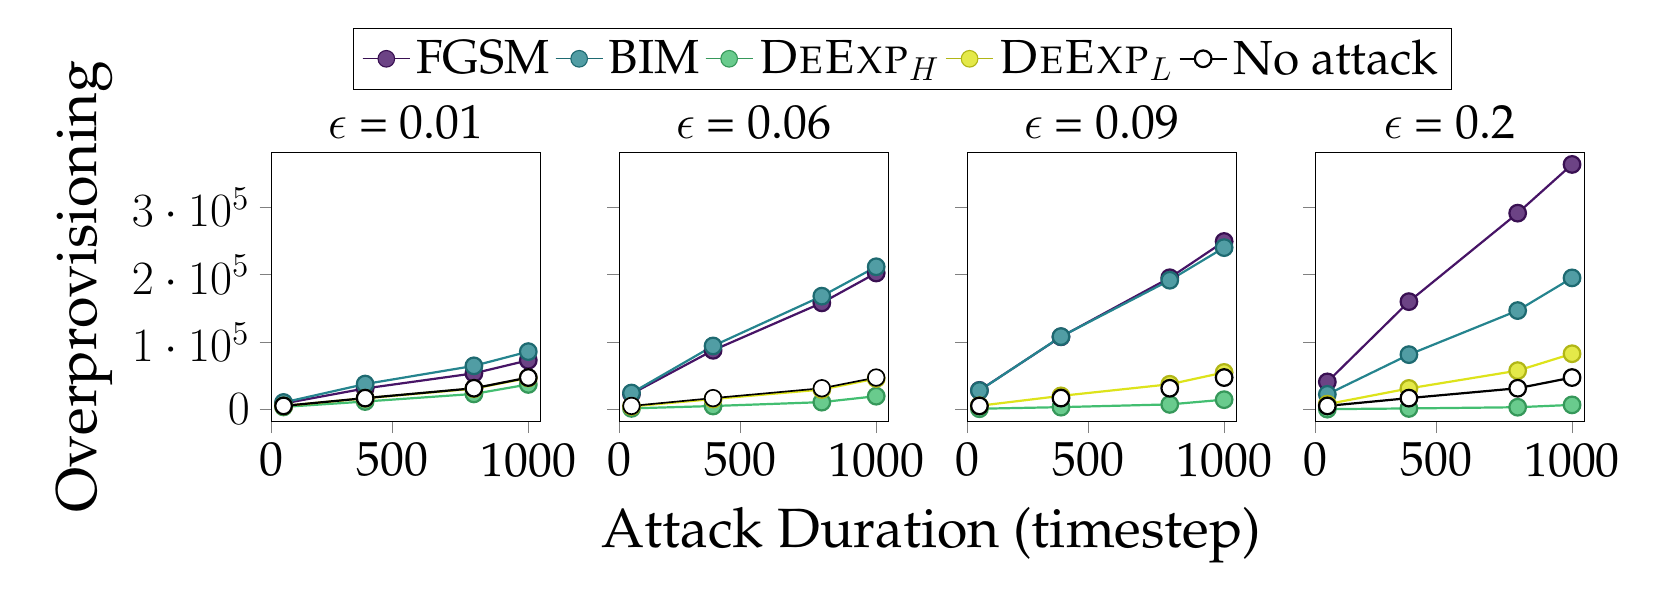
\begin{tikzpicture}

\definecolor{darkgray176}{RGB}{176,176,176}
\definecolor{green}{RGB}{0,128,0}
\definecolor{lightgray204}{RGB}{204,204,204}
\definecolor{purple}{RGB}{128,0,128}
\definecolor{yellow}{RGB}{255,255,0}

\begin{groupplot}[group style={group size=4 by 1},
	width=5cm, height = 5cm,
	xlabel style={font=\huge},
	ylabel style={font=\huge},
	xticklabel style={font=\LARGE},
	yticklabel style={font=\LARGE},
	title style={font=\LARGE,yshift=-1ex},
	groupplot xlabel = {\fontsize{20}{33} \selectfont Attack Duration (timestep)},
	xtick={55,500,1000},
	xticklabels={0,500,1000},
	yticklabel style={%
		scaled y ticks = false,
		/pgf/number format/.cd,
	},
	xticklabel style={%
		scaled y ticks = false,
		/pgf/number format/.cd,
		fixed,
		precision=0,
		fixed zerofill,
		1000 sep={\,},
	},colormap/viridis
	]
\nextgroupplot[
tick align=outside,
tick pos=left,
title={\(\displaystyle \epsilon\) = 0.01},
xmin=55, xmax=1045,
ylabel={Overprovisioning},
ymin=-17815.9055, ymax=381862.1755,
]
\addplot [thick, normal-color={50}, mark=*, mark size=3, mark options={solid,fill-color={50}}]
table {%
100 8711.64
400 31086.74
800 53506.11
1000 72850.05
};
\addplot [thick, normal-color={450}, mark=*, mark size=3, mark options={solid,fill-color={450}}]
table {%
100 10287.59
400 37607.61
800 64634.26
1000 85756.87
};
\addplot [thick, normal-color={700}, mark=*, mark size=3, mark options={solid,fill-color={700}}]
table {%
100 3615.47
400 11661.16
800 22966.29
1000 37035.11
};
\addplot [thick, normal-color={950}, mark=*, mark size=3, mark options={solid,fill-color={950}}]
table {%
100 5056.79
400 16474.25
800 30765.62
1000 46653.53
};
\addplot [thick, black, mark=*, mark size=3, mark options={solid, fill=white}]
table {%
100 5142.68
400 16720.63
800 31368.61
1000 47256.14
};

\nextgroupplot[
scaled y ticks=manual:{}{\pgfmathparse{#1}},
tick align=outside,
tick pos=left,
title={\(\displaystyle \epsilon\) = 0.06},
xmin=55, xmax=1045,
ymin=-17815.9055, ymax=381862.1755,
yticklabels={}
]
\addplot [thick, normal-color={50}, mark=*, mark size=3, mark options={solid,fill-color={50}}]
table {%
100 23044.01
400 87675.54
800 158133.44
1000 202499
};
\addplot [thick, normal-color={450}, mark=*, mark size=3, mark options={solid,fill-color={450}}]
table {%
100 24311.94
400 94189.86
800 168114.67
1000 211748.7
};
\addplot [thick, normal-color={700}, mark=*, mark size=3, mark options={solid,fill-color={700}}]
table {%
100 1467.62
400 4979.52
800 10735.84
1000 19579.17
};
\addplot[thick, normal-color={950}, mark=*, mark size=3, mark options={solid,fill-color={950}}]
table {%
100 4406.84
400 15304.15
800 29476.53
1000 45802.69
};
\addplot [semithick, black, mark=*, mark size=3, mark options={solid, fill=white}]
table {%
100 5142.68
400 16720.63
800 31368.61
1000 47256.14
};

\nextgroupplot[
scaled y ticks=manual:{}{\pgfmathparse{#1}},
tick align=outside,
tick pos=left,
title={\(\displaystyle \epsilon\) = 0.09},
xmin=55, xmax=1045,
ymin=-17815.9055, ymax=381862.1755,
yticklabels={}
]
\addplot [thick, normal-color={50}, mark=*, mark size=3, mark options={solid,fill-color={50}}]
table {%
100 28165.99
400 107757.18
800 195408.1
1000 249303.24
};
\addplot [thick, normal-color={450}, mark=*, mark size=3, mark options={solid,fill-color={450}}]
table {%
100 27914.73
400 108069.83
800 191732.28
1000 240195.39
};
\addplot [thick, normal-color={700}, mark=*, mark size=3, mark options={solid,fill-color={700}}]
table {%
100 941.76
400 3323.32
800 7392.74
1000 14411.46
};
\addplot [thick, normal-color={950}, mark=*, mark size=3, mark options={solid,fill-color={950}}]
table {%
100 5386.69
400 20036.28
800 37285.92
1000 54846.92
};
\addplot [thick, black, mark=*, mark size=3, mark options={solid,fill=white}, only marks]
table {%
100 5142.68
400 16720.63
800 31368.61
1000 47256.14
};

\nextgroupplot[
scaled y ticks=manual:{}{\pgfmathparse{#1}},
tick align=outside,
tick pos=left,
title={\(\displaystyle \epsilon\) = 0.2},
xmin=55, xmax=1045,
ymin=-17815.9055, ymax=381862.1755,
yticklabels={}
]
\addplot [thick, normal-color={50}, mark=*, mark size=3, mark options={solid,fill-color={50}}]
table {%
100 40798.09
400 159983.05
800 291353.18
1000 363694.99
};
\addplot [thick, normal-color={450}, mark=*, mark size=3, mark options={solid,fill-color={450}}]
table {%
100 22322.26
400 81263.71
800 146718.68
1000 195215.19
};
\addplot [thick, normal-color={700}, mark=*, mark size=3, mark options={solid,fill-color={700}}]
table {%
100 351.28
400 1364.09
800 3193.06
1000 6653.17
};
\addplot [thick, normal-color={950}, mark=*, mark size=3, mark options={solid,fill-color={950}}]
table {%
100 7758.3
400 31080.19
800 57530.07
1000 82614.67
};
\addplot [thick, black, mark=*, mark size=3, mark options={solid, fill=white}]
table {%
100 5142.68
400 16720.63
800 31368.61
1000 47256.14
};
\end{groupplot}
\begin{customlegend}[colormap/viridis,
	legend entries={ % <= in the following there are the entries
		FGSM,
		BIM,
		\textsc{DeExp}$_H$,
		\textsc{DeExp}$_L$,
		No attack,
	},
	legend columns=-1,
	legend style={at={(15,5)},font=\LARGE}] % <= to define position and font legend
	% the following are the "images" and numbers in the legend
	\addlegendimage{fill-color={50}, mark=*, mark size=3, mark options={solid}}
	\addlegendimage{fill-color={450}, mark=*, mark size=3, mark options={solid}}
	\addlegendimage{fill-color={700}, mark=*, mark size=3, mark options={solid}}
	\addlegendimage{fill-color={950}, mark=*, mark size=3, mark options={solid}}
	\addlegendimage{thick,fill=white, draw=black, mark=*, mark size=3, mark options={solid}}
\end{customlegend}
\end{tikzpicture}
\end{document}